% Standalone source. Compile twice with pdflatex.
\documentclass[11pt,a4paper]{article}
\usepackage[T1]{fontenc}
\usepackage{lmodern,microtype,amsmath,amssymb,amsthm,mathtools}
\usepackage[margin=24mm,headheight=15pt]{geometry}
\usepackage{booktabs,array,xcolor,fancyhdr,titlesec,fancyvrb,tikz}
\usepackage[colorlinks=true,linkcolor=teal!65!black,citecolor=teal!65!black,urlcolor=teal!65!black]{hyperref}
\definecolor{ink}{HTML}{15364A}
\definecolor{accent}{HTML}{007C78}
\titleformat{\section}{\Large\sffamily\bfseries\color{ink}}{\thesection}{.55em}{}
\titleformat{\subsection}{\large\sffamily\bfseries\color{accent}}{\thesubsection}{.55em}{}
\newtheorem{theorem}{Theorem}[section]
\newtheorem{lemma}[theorem]{Lemma}
\newtheorem{proposition}[theorem]{Proposition}
\newtheorem{corollary}[theorem]{Corollary}
\theoremstyle{remark}
\newtheorem{remark}[theorem]{Remark}
\DeclareMathOperator{\conv}{conv}
\DeclareMathOperator{\vol}{vol}
\DeclareMathOperator{\Vol}{Vol}
\DeclareMathOperator{\inter}{int}
\newcommand{\R}{\mathbb R}\newcommand{\Z}{\mathbb Z}
\newcommand{\fr}[1]{\left\{#1\right\}}
\newcommand{\one}{\mathbf1}
\pagestyle{fancy}\fancyhf{}
\fancyhead[L]{\small\sffamily Weighted terminal simplices}
\fancyhead[R]{\small\sffamily Exact counterexamples}
\fancyfoot[L]{\footnotesize\sffamily Research draft | 20 November 2026}
\fancyfoot[R]{\small\thepage}
\setlength{\parindent}{1.1em}\setlength{\parskip}{3pt}
\setlength{\emergencystretch}{2em}\raggedbottom
\hypersetup{pdftitle={Weighted Terminal Simplices: Counterexamples and Exact Covering Minima},pdfauthor={Research note prepared for Keio}}

\begin{document}
\noindent{\sffamily\small\bfseries\color{accent} GEOMETRY OF NUMBERS | TRANSFER FROM VMRC [200]}\par\medskip
\noindent{\sffamily\bfseries\fontsize{23}{27}\selectfont\color{ink}
Weighted Terminal Simplices:\\
Counterexamples and\\
Exact Covering Minima\par}
\medskip
\noindent{\large\sffamily Non-coordinate projections, a minimal-dimensional extremizer,\par
and equality obstructions with any number of interior points}\par
\medskip
\noindent Research note prepared for Keio\hfill 20 November 2026

\begin{abstract}
We give explicit counterexamples to Conjecture 5.3 of
Codenotti--Santos--Schymura on the covering minima of weighted terminal
simplices. For every real $r>1$, the tetrahedron
$K_r=S(1,1,r,r)$ has a rank-two lattice quotient with covering radius
$\tfrac12+\tfrac1{r+1}$, strictly exceeding the conjectured value
$(r+2)/(2r+1)$. For every integer $m\ge2$, a previously proved planar
covering theorem bounds every rank-two quotient and gives the exact value
$\mu_2(K_m)=\tfrac12+\tfrac1{m+1}$. Thus the conjecture already fails
in the smallest possible ambient dimension, three; the example
$S(1,1,2,2)$ has $\mu_2=5/6$, rather than $4/5$.
The construction was obtained by transferring the weighted fractional-part
method of VMRC [200]. We supply an elementary independent proof of the
counterexample and a separate exact fractional-part certificate.
We also reduce the equality-classification counterexample from [200]
to the smallest possible dimension, four, and obtain five-dimensional
counterexamples to the equality clause of Conjecture D for every integer
$k\ge2$. The numerical upper bound of Conjecture D in general dimension
is not addressed.
\end{abstract}

\section{The original conjecture and the results}
For a convex body $K\subset\R^d$ and a full-rank lattice $\Lambda$, write
\[
 \mu(K,\Lambda)=\inf\{\rho\ge0:\rho K+\Lambda=\R^d\}.
\]
The $i$th covering minimum $\mu_i(K,\Lambda)$ is the infimum of the
dilations $\rho$ for which $\rho K+\Lambda$ intersects every affine
subspace of codimension $i$. In particular $\mu_d=\mu$.
We use the standard quotient description \cite[Section 1]{CSS}:
\begin{equation}\label{eq:quotient}
 \mu_i(K,\Lambda)=\sup_{A}\mu(AK,A\Lambda),
\end{equation}
where $A$ runs over rank-$i$ linear quotients with rational kernel
relative to $\Lambda$. Then $A\Lambda$ is a full-rank lattice in the
quotient. Identifying the quotient with $\R^i$ by a linear isomorphism
does not change its covering radius. This formulation also accounts
for the irrational affine subspaces in the original definition.

For $\omega\in\R_{>0}^{d+1}$, define
\[
 S(\omega)=\conv\{-\omega_0\one_d,\omega_1e_1,\ldots,\omega_de_d\}.
\]
Codenotti--Santos--Schymura \cite[Conjecture 5.3]{CSS} proposed that,
when $\omega_0\le\cdots\le\omega_d$,
\begin{equation}\label{eq:conjecture}
 \mu_i(S(\omega),\Z^d)=
 \frac{\displaystyle\sum_{0\le j<k\le i}(\omega_j\omega_k)^{-1}}
      {\displaystyle\sum_{j=0}^{i}\omega_j^{-1}}.
\end{equation}
Equivalently, the maximal quotient radius would be attained by a
projection onto the first $i$ coordinates. The same statement is
Conjecture 5.3 in Krivoku\'ca's January 2026 paper \cite{Krivokuca}.

\begin{theorem}[Failure for every real parameter $r>1$]\label{thm:real}
Let
\[
 K_r=S(1,1,r,r)=\conv\{(-1,-1,-1),e_1,re_2,re_3\}\subset\R^3.
\]
For every real $r>1$,
\begin{equation}\label{eq:real}
 \mu_2(K_r,\Z^3)\ \ge\ \frac12+\frac1{r+1}
 \ >\ \frac{r+2}{2r+1}.
\end{equation}
Consequently \eqref{eq:conjecture} is false. The strict gap between the
displayed lower bound and the conjectured value is
\begin{equation}\label{eq:gap}
 \frac{r-1}{2(r+1)(2r+1)}.
\end{equation}
\end{theorem}

\begin{theorem}[Exact values for the infinite integer family]\label{thm:integer}
For every integer $m\ge2$,
\begin{equation}\label{eq:integer}
 \boxed{\mu_2(K_m,\Z^3)=\frac12+\frac1{m+1}.}
\end{equation}
In particular, $\mu_2(S(1,1,2,2))=5/6$, whereas
\eqref{eq:conjecture} predicts $4/5$.
\end{theorem}

The proofs of these two theorems are in Sections 2--3. No assertion
of equality in \eqref{eq:real} is made for arbitrary noninteger $r$.
The cases $i=1$ and $i=d$ of the original conjecture are theorems
\cite[Theorem 1.4 and the discussion after Conjecture 5.3]{CSS}.
Thus dimension three is the smallest ambient dimension in which
the conjecture can fail.

\section{An explicit quotient and an elementary global lower bound}
Consider the integer linear map
\begin{equation}\label{eq:A}
 A(x_1,x_2,x_3)=(x_2+x_3,x_1).
\end{equation}
It is surjective on lattices: $A\Z^3=\Z^2$. Its image on the
tetrahedron is
\begin{equation}\label{eq:Pr}
 P_r=AK_r=\conv\{(-2,-1),(r,0),(0,1)\}.
\end{equation}
The affine lattice isomorphism
\[
 T(x,y)=(y,x-y+1)
\]
has linear determinant $-1$ and maps the three displayed vertices to
$(-1,0),(0,r+1),(1,0)$, respectively. Covering radius is invariant
under translations of the body and under simultaneous lattice-linear
isomorphisms. Hence
\begin{equation}\label{eq:Qr}
 \mu(P_r,\Z^2)=\mu(Q_{r+1},\Z^2),\qquad
 Q_L=\conv\{(-1,0),(1,0),(0,L)\}.
\end{equation}

\begin{lemma}[A triangular covering radius]\label{lem:triangle}
For every real $L>0$,
\[
 \mu(Q_L,\Z^2)=\frac12+\frac1L.
\]
\end{lemma}
\begin{proof}
At height $y=f\ge0$, the horizontal section of $\rho Q_L$ is
\[
 |x|\le\rho-f/L,
\]
when the right-hand side is nonnegative. For any point of the plane,
subtract an integer from its second coordinate to obtain
$f\in[0,1)$, and subtract a nearest integer from its first coordinate
to obtain $|x|\le1/2$. If $\rho=1/2+1/L$, then
$\rho-f/L\ge1/2$, proving the covering upper bound.

Conversely, suppose $\rho<1/2+1/L$. Choose $f\in[0,1)$ such that
$\rho<1/2+f/L$, and consider $(1/2,f)$. In any possible translate of
$\rho Q_L$ containing it, the residual second coordinate is
$f+j\ge f$ for an integer $j\ge0$, since $Q_L$ has no negative
second coordinates. The corresponding horizontal half-length is at
most $\rho-f/L<1/2$, whereas the distance of $1/2$ from every integer
is at least $1/2$. No such translate exists. This proves the reverse
inequality.
\end{proof}

The lemma is also the known direct-sum formula applied to
$[-1,1]\oplus[0,L]$ \cite[Corollary 2.2]{CSS}; its elementary proof
is included to make the counterexample independently checkable.

\begin{proof}[Proof of Theorem~\ref{thm:real}]
Equations \eqref{eq:quotient}--\eqref{eq:Qr} and
Lemma~\ref{lem:triangle} give
\[
 \mu_2(K_r,\Z^3)\ge\mu(P_r,\Z^2)=\frac{r+3}{2(r+1)}.
\]
For the ordered weights $(1,1,r,r)$, the proposed value for $i=2$ is
\[
 \frac{1+2/r}{2+1/r}=\frac{r+2}{2r+1}.
\]
Subtracting yields \eqref{eq:gap}, which is positive for every $r>1$.
This establishes a global counterexample family with no numerical
approximation.
\end{proof}

\section{The upper bound over every quotient for integer weights}
We use a previously proved planar theorem, rather than an unproved
general-dimensional conjecture.

\begin{theorem}[Codenotti--Santos--Schymura]\label{thm:planar}
If a lattice polygon $P$ has exactly $k\ge2$ interior lattice points,
then
\[
 \mu(P,\Lambda)\le\frac12+\frac1{k+1}.
\]
\end{theorem}
This is \cite[Theorem 6.3]{CSS}, applied in a basis of the ambient
lattice $\Lambda$.

\begin{lemma}[Interior lattice chains]\label{lem:chains}
For an integer $m\ge2$, both chains
\[
 \{je_2:0\le j\le m-1\},\qquad
 \{je_3:0\le j\le m-1\}
\]
lie in $\inter K_m$.
\end{lemma}
\begin{proof}
For $je_2$, put
\[
 a=\frac{m-j}{2(m+1)}>0.
\]
Its barycentric coefficients relative to
$(-1,-1,-1),e_1,me_2,me_3$ are
\[
 a,\quad a,\quad (j+a)/m,\quad a/m.
\]
They are all positive, sum to one, and give $je_2$.
Interchanging the last two coordinates proves the other chain.
\end{proof}

\begin{proof}[Proof of Theorem~\ref{thm:integer}]
Let $B:\R^3\to\R^2$ be any rank-two quotient with rational kernel,
and set $\Lambda_B=B\Z^3$. Both $Be_2$ and $Be_3$ cannot vanish:
otherwise the image of $B$ would be spanned by $Be_1$ and have rank
at most one. Choose a nonzero $v$ among $Be_2,Be_3$.

By Lemma~\ref{lem:chains}, the polygon $BK_m$ contains the $m$
distinct points $0,v,\ldots,(m-1)v$ in its interior. Interior points
remain interior under a surjective linear map, since such a map is
open. The polygon is a lattice polygon for $\Lambda_B$.
If it has $k$ interior lattice points, then $k\ge m$ and
Theorem~\ref{thm:planar} gives
\[
 \mu(BK_m,\Lambda_B)\le\frac12+\frac1{k+1}
 \le\frac12+\frac1{m+1}.
\]
This holds for every admissible quotient. Taking the supremum in
\eqref{eq:quotient} proves the upper bound. The specific map $A$ of
\eqref{eq:A} attains it, by Lemma~\ref{lem:triangle}.
\end{proof}

\begin{corollary}[The complete covering-minima vector]\label{cor:vector}
For every integer $m\ge2$,
\[
 \left(\mu_1(K_m),\mu_2(K_m),\mu_3(K_m)\right)
 =\left(\frac12,\frac{m+3}{2(m+1)},
        \frac{m^2+4m+1}{2m(m+1)}\right).
\]
\end{corollary}
\begin{proof}
The first and last values are the known endpoint formulas of
\cite[Theorem 1.4 and the paragraph after Conjecture 5.3]{CSS}.
For the last, substitute the reciprocal weights $(1,1,1/m,1/m)$.
The middle value is Theorem~\ref{thm:integer}.
\end{proof}

\begin{center}
\begin{tabular}{@{}ccccc@{}}
\toprule
$m$ & $\mu_1$ & Actual $\mu_2$ & Conjectured $\mu_2$ & $\mu_3$\\
\midrule
2 & $1/2$ & $5/6$ & $4/5$ & $13/12$\\
3 & $1/2$ & $3/4$ & $5/7$ & $11/12$\\
4 & $1/2$ & $7/10$ & $2/3$ & $33/40$\\
\bottomrule
\end{tabular}
\end{center}

\section{The exact transfer from fractional-part flows}
This section explains how the construction arises from VMRC [200]
\cite{VMRC200}. The counterexample proof in Section 2 is independent
of that manuscript's general covering theorem.

\subsection{An exact weighted gauge formula}
Let $u_0,\ldots,u_d\in\Lambda$ generate the full lattice $\Lambda$,
and suppose their column matrix $U$ has rank $d$ and kernel
$\R q$, where $q_j$ are positive integers. For positive real $c_j$, set
\[
 P=\conv(u_0/c_0,\ldots,u_d/c_d).
\]
The positive relation ensures $0\in\inter P$.

\begin{lemma}[Weighted fractional-part equivalence]\label{lem:gauge}
For every $x=Ut$,
\begin{equation}\label{eq:gauge}
 \inf_{z\in\Lambda}\inf\{\rho\ge0:x-z\in\rho P\}
 =\min_{s\in[0,1)}\sum_{j=0}^d c_j\fr{t_j+sq_j}.
\end{equation}
\end{lemma}
\begin{proof}
Write $z=Un$, $n\in\Z^{d+1}$. Every coefficient representation of
$x-z$ in the columns of $U$ is $t-n+sq$. Its contribution to the
gauge of $P$ is the sum $\sum c_j(t_j-n_j+sq_j)$, subject to all
coefficients being nonnegative. For fixed $s$, each $n_j$ is therefore
at most $\lfloor t_j+sq_j\rfloor$, and choosing those largest values
minimizes the sum. Infima over $s$ and $n$ can be interchanged.
The resulting function is one-periodic and increases strictly
between finitely many jumps, so its minimum is attained at a jump.
\end{proof}

The lattice-generation hypothesis concerns the columns $u_j$, not
the scaled vertices $u_j/c_j$. This distinction matters for $P_2$.

\begin{lemma}[The jump-square upper bound]\label{lem:jump}
With $C=\sum q_jc_j$, every phase vector $t$ satisfies
\[
 \min_s\sum_jc_j\fr{t_j+sq_j}
 \le\frac12\sum_jc_j-\frac{\sum_jq_jc_j^2}{2C}.
\]
\end{lemma}
\begin{proof}
Write $F(s)=\sum c_j\{t_j+sq_j\}$ and let $J_e$ be the total
downward jump at an event $e$, grouping simultaneous crossings.
Between events $F'=C$. Over one period,
\[
 \int_0^1F(s)\,ds=\tfrac12\sum c_j,\qquad
 \sum_eJ_e=C.
\]
The total change of $F^2$ is zero. At an event it is
$-2J_eF(e)-J_e^2$, using the right-continuous value. Consequently
\[
 \frac1C\sum_eJ_eF(e)
 =\frac12\sum_jc_j-\frac1{2C}\sum_eJ_e^2
 \le\frac12\sum_jc_j-\frac1{2C}\sum_jq_jc_j^2.
\]
The left side is a convex combination of the event values.
The last inequality follows from positivity of all weights,
including at simultaneous events.
\end{proof}

\subsection{A finite certificate for the smallest integral example}
For $P_2=\conv((-2,-1),(2,0),(0,1))$, take
\[
 (u_0,u_1,u_2)=((-2,-1),(1,0),(0,1)),\quad
 q=(1,2,1),\quad c=(1,1/2,1),
\]
and
\[
 t=(-1/3,0,-5/6),\qquad x_*=Ut=(2/3,-1/2).
\]
The function in \eqref{eq:gauge} is
\begin{equation}\label{eq:F}
 F(s)=\{s-1/3\}+\tfrac12\{2s\}+\{s-5/6\}.
\end{equation}
Its events are $0,1/3,1/2,5/6$. At every event $F=5/6$, and between
events its slope is $3$. Thus its global minimum is exactly $5/6$.
Lemma~\ref{lem:jump} also gives the uniform upper bound
$\tfrac12(5/2)-\tfrac1{6}(5/2)=5/6$ for every phase.
This proves $\mu(P_2)=5/6$ directly in the framework of [200].

\begin{figure}[ht]
\centering
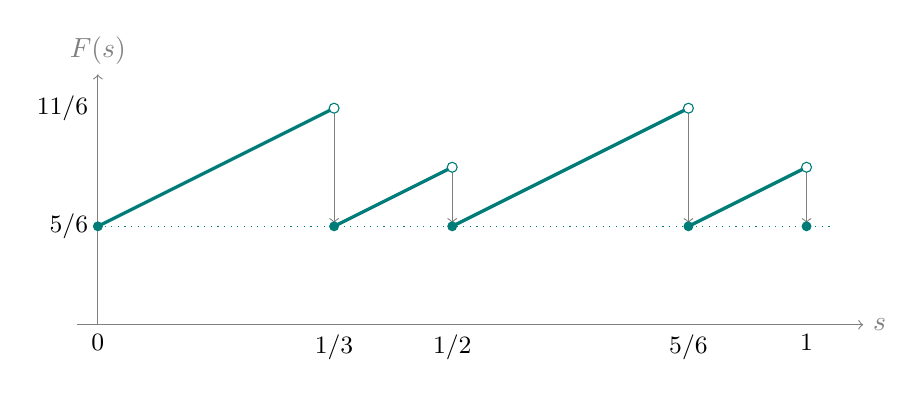
\begin{tikzpicture}[x=9cm,y=1.5cm]
 \draw[->,gray] (-.03,0)--(1.08,0) node[right]{$s$};
 \draw[->,gray] (0,0)--(0,2.12) node[above]{$F(s)$};
 \draw[dotted,accent] (0,.833333)--(1.04,.833333);
 \draw[very thick,accent] (0,.833333)--(.333333,1.833333);
 \draw[very thick,accent] (.333333,.833333)--(.5,1.333333);
 \draw[very thick,accent] (.5,.833333)--(.833333,1.833333);
 \draw[very thick,accent] (.833333,.833333)--(1,1.333333);
 \foreach \x/\y in {.333333/1.833333,.5/1.333333,.833333/1.833333,1/1.333333}{
  \draw[->,gray] (\x,\y)--(\x,.86);
  \draw[accent,fill=white] (\x,\y) circle(1.8pt);}
 \foreach \x in {0,.333333,.5,.833333,1}{\fill[accent] (\x,.833333) circle(1.8pt);}
 \foreach \x/\lab in {0/0,.333333/{1/3},.5/{1/2},.833333/{5/6},1/1}{
  \node[below,font=\small] at (\x,0){$\lab$};}
 \node[left,font=\small] at (0,.833333){$5/6$};
 \node[left,font=\small] at (0,1.833333){$11/6$};
\end{tikzpicture}
\caption{The exact certificate \eqref{eq:F}. Every post-jump value is
$5/6$; positivity of the intervening slope controls every real $s$.}
\end{figure}

There is also a short independent integer certificate. The gauge of
$P_2$ is
\[
 g_{P_2}(x,y)=\max\{x/2+y,\ -x+y,\ x/2-2y\}.
\]
If $x_*-(h,k)\in\rho P_2$ for integers $h,k$ and $\rho<5/6$,
the three inequalities imply
\[
 h+2k\ge-1,\qquad h-k\le1,\qquad h-4k\ge2.
\]
The first two force $k\ge0$, while the last two force $k\le-1$.
This contradiction excludes \emph{every} lattice translate.

\section{A four-dimensional equality counterexample}
We next strengthen the equality-classification counterexample of
VMRC [200]. Let
\begin{equation}\label{eq:S4}
 S=\conv\{(-2,-1,-1,-1),e_1,e_2,e_3,e_4\}\subset\R^4.
\end{equation}

\begin{theorem}[Smallest possible counterexample dimension]\label{thm:S4}
The simplex $S$ has $0\in\inter S$, normalized volume $6$, and
$\mu(S,\Z^4)=2$. It is not obtained from standard terminal simplices
by translations and direct sums, up to unimodular equivalence.
It therefore disproves the equality clause of Conjecture A in
dimension four. This is the smallest possible dimension.
\end{theorem}
\begin{proof}
Write $v_0=(-2,-1,-1,-1)$, $v_j=e_j$ for $j\ge1$. The positive
primitive relation is $q=(1,2,1,1,1)$, with sum $Q=6$. Its normalized
coefficients give strictly positive barycentric coordinates for zero.
The standard basis vertices generate the whole lattice.

The residue classes
\[
 1\pmod6,\quad0\pmod3,\quad2\pmod6,\quad4\pmod6,\quad5\pmod6
\]
partition the integers. Choose
\[
 t=(-1/6,0,-1/3,-2/3,-5/6).
\]
There is exactly one crossing at each $s=j/6$, and
\begin{equation}\label{eq:S4cert}
 \sum_{j=0}^4\{t_j+q_js\}=2+\{6s\}\qquad(s\in\R).
\end{equation}
Both sides have slope $6$, the same unit jumps, and value $2$ at zero,
which proves the all-real identity including its endpoints.
Lemma~\ref{lem:gauge} gives the global lower bound $2$ at
\[
 x_*=(1/3,-1/6,-1/2,-2/3).
\]
Lemma~\ref{lem:jump}, with all $c_j=1$, gives the matching upper bound
for every point.

Using edges from $v_0$, the normalized volume is
\[
 \det(I_4+(2,1,1,1)^{\mathsf T}\one_4^{\mathsf T})=6.
\]
A standard terminal $j$-simplex has normalized volume $j+1$.
Translations preserve volume and direct sums multiply normalized
volumes. Thus a body in the proposed family of dimension four has
volume in
\[
 \{5,8,9,12,16\},
\]
as obtained from the five integer partitions of four. Volume six is
excluded. These invariants are unchanged by unimodular maps.
Finally, the complete equality classification is already proved
in dimensions at most three \cite[Theorem 1.3]{CSS}.
\end{proof}

For clarity, the volume multiplication used here remains valid when
the origin is on the boundary of a summand. For bodies of dimensions
$a,b$, the fiber formula for their free sum gives
\[
 \vol_{a+b}(K\oplus L)
 =\frac{a!b!}{(a+b)!}\vol_a(K)\vol_b(L),
\]
by integrating the scaled fibers $(1-g_K(x))L$ over $K$.
The sublevel volume of the possibly extended gauge $g_K$ is
$t^a\vol_a(K)$; the beta integral proves the displayed identity.
Multiplication by $(a+b)!$ gives normalized-volume multiplication.

\section{Equality counterexamples with every prescribed \texorpdfstring{$k\ge2$}{k >= 2}}
Conjecture D of \cite{CSS} proposes, for a lattice $d$-polytope with
$k\ge1$ interior lattice points,
\[
 \mu(P)\le\frac{d-1}{2}+\frac1{k+1},
\]
and specifies an equality family. For $k\ge2$ that family is formed
from a segment of length $k+1$ and standard terminal simplices by
translations and direct sums. The following result concerns its
\emph{equality clause}, not the general numerical upper bound.

\begin{theorem}[Five-dimensional counterexamples for all $k\ge2$]
\label{thm:D}
For the simplex $S$ in \eqref{eq:S4}, put
\[
 R_k=S\oplus[-1,k]\subset\R^4\oplus\R,\qquad k\in\Z,\ k\ge2.
\]
Then
\[
 |\inter R_k\cap\Z^5|=k,\qquad
 \mu(R_k,\Z^5)=2+\frac1{k+1},\qquad
 \Vol_{\Z^5}(R_k)=6(k+1).
\]
No $R_k$ belongs to the equality family proposed in Conjecture D.
\end{theorem}
\begin{proof}
The facet inequalities of $S$ are $\ell_j(x)\le1$, where
\begin{align*}
 \ell_0(x)&=x_1+x_2+x_3+x_4,\\
 \ell_1(x)&=-2x_1+x_2+x_3+x_4,\\
 \ell_2(x)&=x_1-5x_2+x_3+x_4,\\
 \ell_3(x)&=x_1+x_2-5x_3+x_4,\\
 \ell_4(x)&=x_1+x_2+x_3-5x_4.
\end{align*}
They satisfy $\ell_0+2\ell_1+\ell_2+\ell_3+\ell_4=0$.
For an interior lattice point, all these integer-valued forms are
nonpositive, so positivity of the relation forces all to be zero;
their common kernel is zero. Thus zero is the only interior lattice
point of $S$. More precisely its gauge
$g_S(z)=\max_j\ell_j(z)$ is an integer at every $z\in\Z^4$ and
is at least one when $z\ne0$.

The gauge of a free sum is the sum of the two gauges. A lattice point
$(z,t)$ can therefore be in $\inter R_k$ only if $z=0$. For $z=0$,
the permitted integers are precisely $-1<t<k$, namely
$0,1,\ldots,k-1$. This proves the count.

For a direct-product lattice, minimizing the sum gauge over lattice
translates separates in the two factors. Taking the two independent
suprema yields additivity of covering radii, also stated in
\cite[Corollary 2.2]{CSS}. Hence
$\mu(R_k)=\mu(S)+\mu([-1,k])=2+1/(k+1)$.
The normalized-volume identity gives $6(k+1)$.

If $R_k$ were in the proposed family, the terminal-simplex factors
would have dimensions with total four and volumes with product six,
after canceling the common segment factor $k+1$. The possible
products in dimension four are $5,8,9,12,16$, none equal to six.
This excludes all permitted translations, direct-sum groupings and
unimodular images.
\end{proof}

\section{Scope, dependence, and historical status}
The principal outcome is the failure of the original weighted
covering-minima conjecture, together with an exact formula for all
integer members of $S(1,1,m,m)$. The lower-bound counterexample uses
only an explicit lattice quotient, an affine lattice isomorphism,
and the elementary triangle computation. The exact upper bound for
integer parameters uses the \emph{proved planar} theorem of CSS.
The auxiliary equality counterexamples have complete fractional-part
and volume proofs above.

The underlying general transfer method comes from VMRC [200].
The present note adds the specific non-coordinate quotient, the
counterexample family, the global integer-parameter upper bound,
and the lower-dimensional equality constructions. The endpoint
covering-minima formulas, the planar theorem and the direct-sum
covering formula are prior results and are credited accordingly.

The original conjecture is present in the 2019 preprint and the
2022 journal article \cite{CSS}; it is explicitly repeated in the
2026 preprint \cite{Krivokuca}. Searches of the original and recent
primary sources and searches for the conjecture with counterexample
terms did not identify the same resolution as of 20 November 2026.
This is a bounded search report. Historical priority and publication
status require independent specialist assessment.

This note does not determine $\mu_2(K_r)$ for every noninteger $r$,
classify all weighted terminal-simplex covering minima, prove the
general covering-product conjecture, or settle the numerical
Conjecture D in higher dimension. These remaining questions are
separate from the universal conjectures refuted above.

\appendix
\section{Exact-arithmetic certificate code}
The following standalone Python 3 code uses only rational arithmetic.
It checks the explicit projection, the event certificates and the
small volume obstruction. The proofs for all parameters are in the
main text; sampling parameter values is not used as their justification.
\begin{Verbatim}[fontsize=\footnotesize,frame=single]
from fractions import Fraction as F
from itertools import combinations

def frac(x):
    return x - x.numerator // x.denominator

def flow(q, c, t):
    events = set()
    for r, a in zip(q, t):
        for j in range(r):
            events.add(frac((F(j)-a)/r))
    values = {s: sum(w*frac(a+r*s)
                    for r,w,a in zip(q,c,t)) for s in events}
    C = sum(r*w for r,w in zip(q,c))
    B = (sum(c)-sum(r*w*w for r,w in zip(q,c))/C)/2
    return events, values, B

def project(v):
    return (v[1]+v[2], v[0])

def affine(v):
    x,y = v
    return (y,x-y+1)

vertices = [(-1,-1,-1),(1,0,0),(0,2,0),(0,0,2)]
image = set(map(project,vertices))
assert image == {(-2,-1),(0,1),(2,0)}
assert set(map(affine,image)) == {(-1,0),(1,0),(0,3)}

q = [1,2,1]
c = [F(1),F(1,2),F(1)]
t = [-F(1,3),F(0),-F(5,6)]
E,V,B = flow(q,c,t)
assert E == {F(0),F(1,3),F(1,2),F(5,6)}
assert set(V.values()) == {F(5,6)} and B == F(5,6)
assert F(5,6)-F(4,5) == F(1,30)

for m in [2,3,4,10]:
    actual = F(1,2)+F(1,m+1)
    predicted = F(m+2,2*m+1)
    assert actual-predicted == F(m-1,2*(m+1)*(2*m+1))
    for j in range(m):
        a = F(m-j,2*(m+1))
        bary = [a,a,(j+a)/m,a/m]
        assert all(x>0 for x in bary) and sum(bary)==1

q4 = [1,2,1,1,1]
t4 = [-F(1,6),F(0),-F(1,3),-F(2,3),-F(5,6)]
E,V,B = flow(q4,[F(1)]*5,t4)
assert E == {F(j,6) for j in range(6)}
assert set(V.values()) == {F(2)} and B == 2
p = [2,1,1,1]
x = [t4[j]-p[j-1]*t4[0] for j in range(1,5)]
assert x == [F(1,3),-F(1,6),-F(1,2),-F(2,3)]
assert 1+sum(p) == 6

def partitions(n, least=1):
    if n == 0:
        yield []
    for k in range(least,n+1):
        for rest in partitions(n-k,k):
            yield [k]+rest

def product(xs):
    a = 1
    for x in xs: a *= x
    return a

volumes = {product(k+1 for k in part) for part in partitions(4)}
assert volumes == {5,8,9,12,16} and 6 not in volumes
print('All exact certificate checks passed.')
\end{Verbatim}

\begin{thebibliography}{9}
\bibitem{CSS}
G.~Codenotti, F.~Santos and M.~Schymura,
\emph{The covering radius and a discrete surface area for non-hollow
simplices}, Discrete \& Computational Geometry \textbf{67} (2022),
65--111. \href{https://doi.org/10.1007/s00454-021-00330-3}
{doi:10.1007/s00454-021-00330-3}.
\href{https://arxiv.org/abs/1903.02866}{arXiv:1903.02866},
v1 (2019), v2 (2021).

\bibitem{Krivokuca}
K.~Krivoku\'ca, \emph{Upper bounds on covering minima of convex bodies},
\href{https://arxiv.org/abs/2601.15173}{arXiv:2601.15173v1},
21 January 2026.

\bibitem{VMRC200}
\emph{Weighted fractional-part flows and sharp lattice covering bounds},
Verifiable Mathematical Reasoning Corpus, manuscript [200],
18 November 2026. Repository revision
\texttt{ac1492a50784be919fe0b5e8f19f96f8d221a22e}.
\href{https://github.com/QEEDDD/Verifiable-Mathematical-Reasoning-Corpus}
{Repository and manuscript source}.
\end{thebibliography}
\end{document}
